
\documentclass{article}

\usepackage{tikz}
\usetikzlibrary{mindmap,trees}
\begin{document}
\pagestyle{empty}


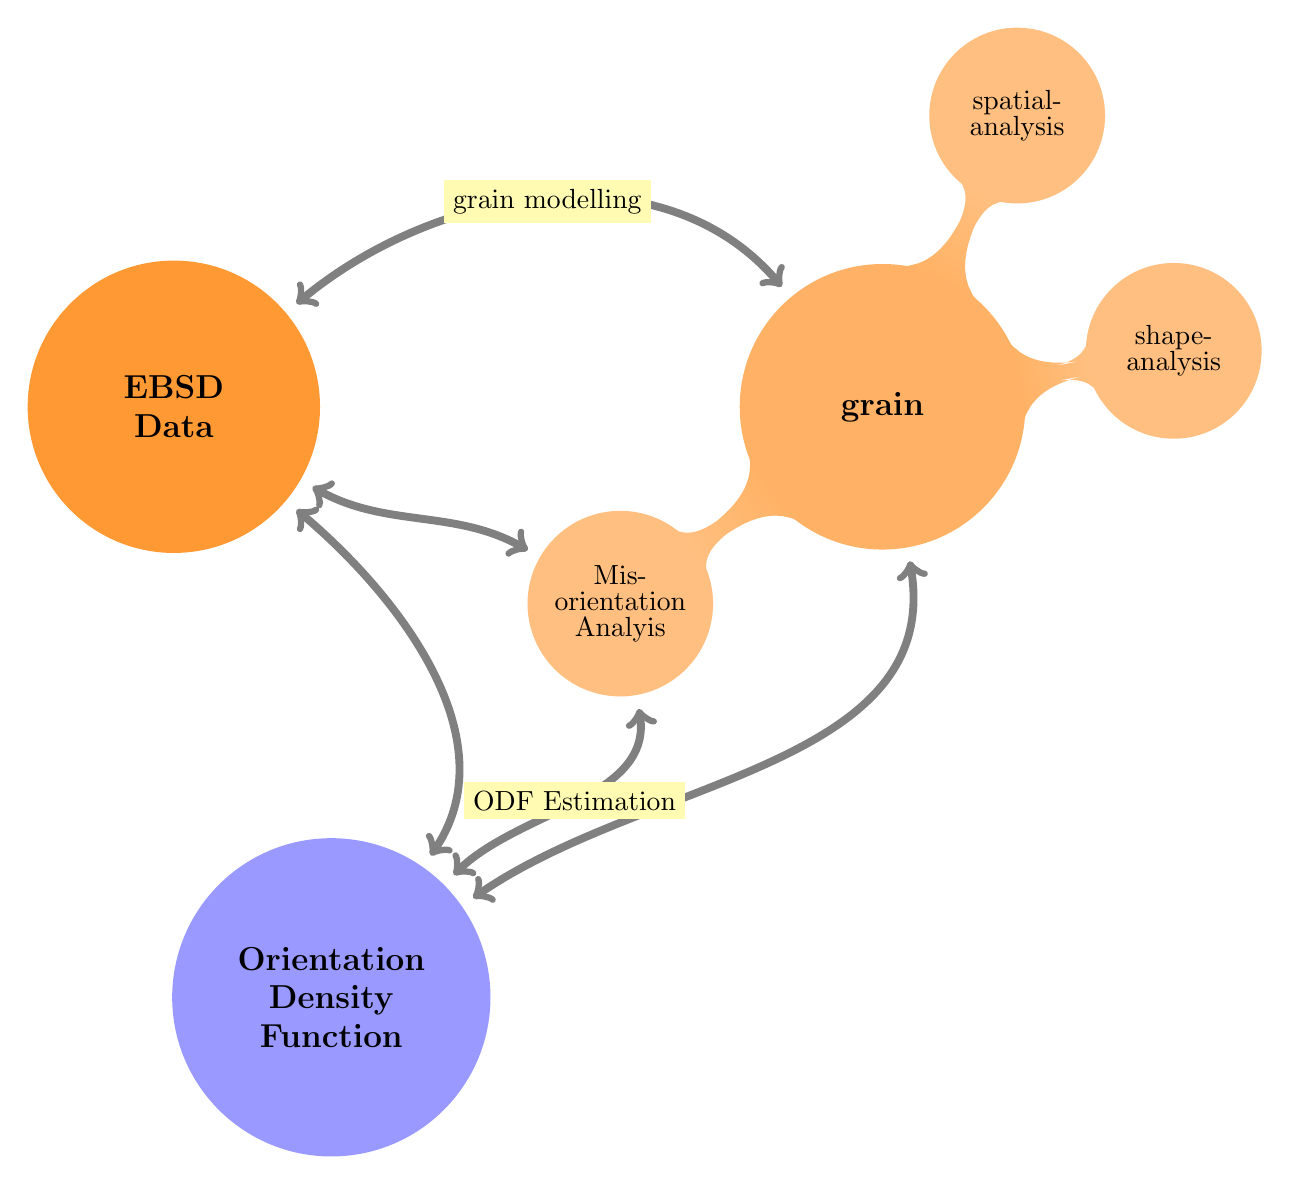
\begin{tikzpicture}[scale = 1]
  \definecolor{myblue}{HTML}{92dcec}
  \tikzstyle{every annotation}=[fill=white, font=\sf]

 \path[mindmap, concept color=orange!80!]
  node[concept,minimum size=3cm](ebsd) at (-4.5,6.5) {\bf EBSD \\Data};
%  child[grow = 20, concept color=orange!50];
  
  \path[mindmap,concept color=orange!60!]
  node[concept,minimum size=3cm](grain) at (4.5,6.5) {\bf grain}
  	child[grow = 20, concept color=orange!50]
	  {	 node[concept, minimum size=1.5cm,font=\footnotesize](pf) at(-1,-1) {\normalsize shape\-analysis}}
	  			child[grow = 70, concept color=orange!50] 
	  {  node[concept,minimum size=1.5cm,font=\footnotesize](pf) at(0,-1) {\normalsize spatial\-analysis}}
	  			child[grow = -150, concept color=orange!50] 
	 	{ node[concept,minimum size=2.3cm,font=\footnotesize](miso) at(1,0) {\normalsize Mis\-orientation Analyis}};
%  child[grow = 20, concept color=orange!50] ;
  
%  
  

  \path[mindmap,concept color=blue!40!]
  node[concept](odf) at (-2.5,-1) {\bf Orientation Density Function};

	\draw [<->,concept connection] (ebsd) to[out=-30,in=150] (miso);
	
	\draw [<->,concept connection] (ebsd) to[out=-40,in=55] (odf); 
	\draw [<->,concept connection] (grain) to[out=-80,in=35] (odf);  
	\draw [<->,concept connection] (miso) to[out=-80,in=45] node[fill=yellow!30] { ODF Estimation}(odf);
	\draw [<->,concept connection] (ebsd) to[out=40,in=130] node[fill=yellow!30] { grain modelling} (grain); 
%	

\end{tikzpicture}

\end{document}
%%% Local Variables: 
%%% mode: latex
%%% TeX-master: t
%%% End: 
